\documentclass{report}
\setcounter{chapter}{0}
\usepackage{graphicx}
%Makes it write "Part" instead of "Chapter" at the beginning of each Chapter
\renewcommand{\chaptername}{Part} 

\begin{document}
\title{CS2006 --- \emph{Core War}}
\author{Chengyi Lin, Ross Apted and Ben Lovell}

\maketitle
\tableofcontents

\chapter{Running instructions}
	\paragraph{}In order to run, run the executable ./Main [warrior 1] [warrior 2] file, which takes 2 arguments for two warrior files.

\chapter{Introduction}
	\section{Aim}
		\paragraph{}The aim of this Project is to implement a core war programming game in which two (or more) programs (known as warriors) battle to control a virtual machine. The warriors are written in a simple programming language called Redcode. The object of the game is to cause the opposing program(s) to terminate, leaving the winning warrior in control of the machine.
	\section{Requirements:}
		\subsection*{Primary requirements}
			\begin{itemize}
				\item Implementing step�, which executes each instruction in the virtual machine. --- Done
				\item Implementing drawSystem in Display.hs which draws a visual representation of the core contents. ---Done
				\item Implementing parsers to convert Strings to instructions. ---Done
				\item Extend main so that it reads two files from the command line, parses them, adds them to the core
and executes the warriors against each other. ---Done
			\end{itemize}
			\paragraph{}Other things for the project were also tackled:
			\subsection*{Secondary Requirements}
			\begin{itemize}
				\item Extend addWarrior so that it adds the warrior to a random location in the core. You will need to make sure that it does not overlap with another warrior. ---Done
			\end{itemize}

\chapter{Description}
	\paragraph{}The program was separated into logically separate parts. This was to allow modularity in the scraping part and the user interface part. 
	\paragraph{}On the one hand, there was the scraping part. This was modularised by using abstract classes and 
		\section{base.py}
			\paragraph{}....
		\section{session.py}
			\paragraph{}....
		\section{Reddit.py}
			\paragraph{}....
		\section{storyview.py}
			\paragraph{}....
		

\chapter{Testing}
	\section{How we Tested}
		\paragraph{}
Used command line to run program tying all possible, cases and took screen shots.
	\section{Tests}
		\begin{itemize}
			\item Basic working, can load two warriors as arguments from command line and run them --- Passed \newline \newline 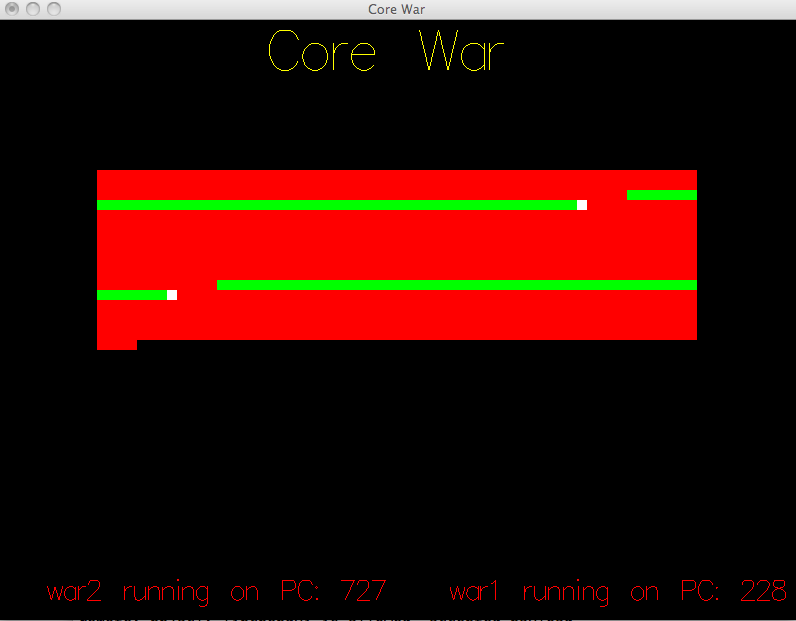
\includegraphics[height=90mm]{1}
			\item Run the given test-state which contains two warriors: dwarf and imp, dwarf win --- Passed  \newline \newline 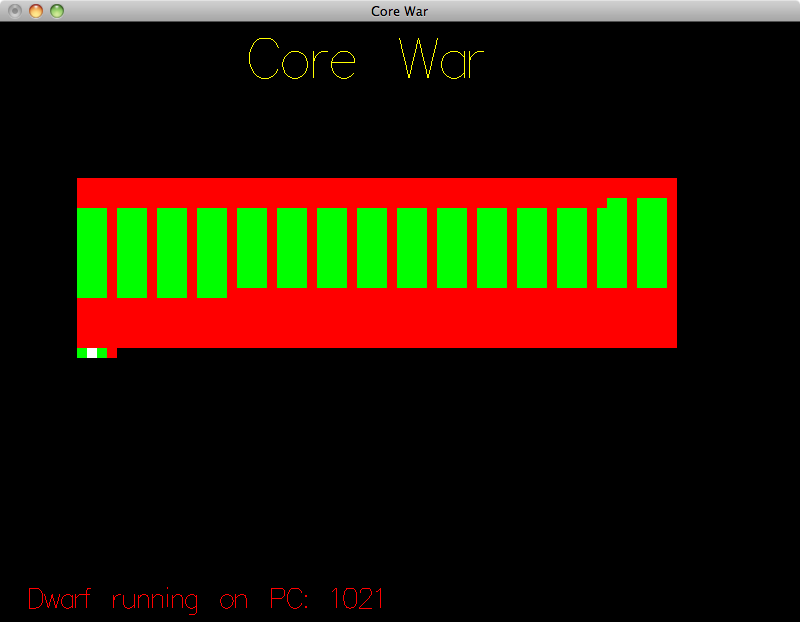
\includegraphics[height=90mm]{2}
			\item Add warriors to random locations --- Passed \newline \newline 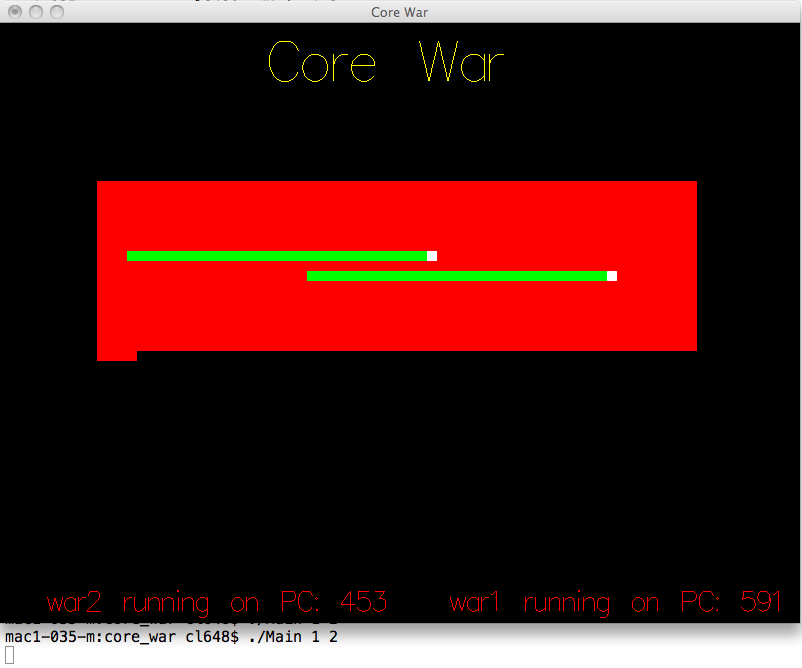
\includegraphics[height=90mm]{3_1} \newline \newline 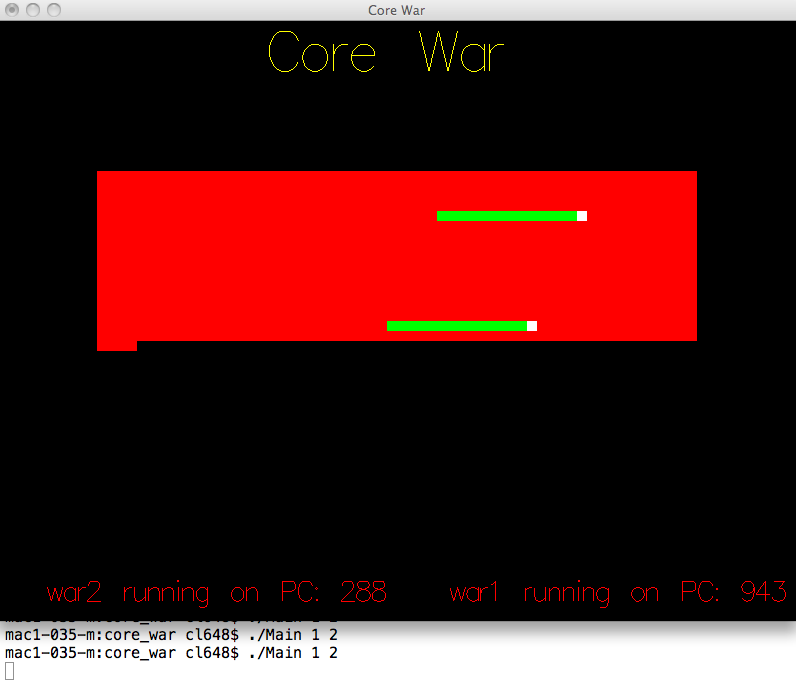
\includegraphics[height=90mm]{3_2}
			\item Never set two warriors to same location (Test by setting the core size to 2, and run program several times, and see if any errors happen) --- Passed \newline \newline 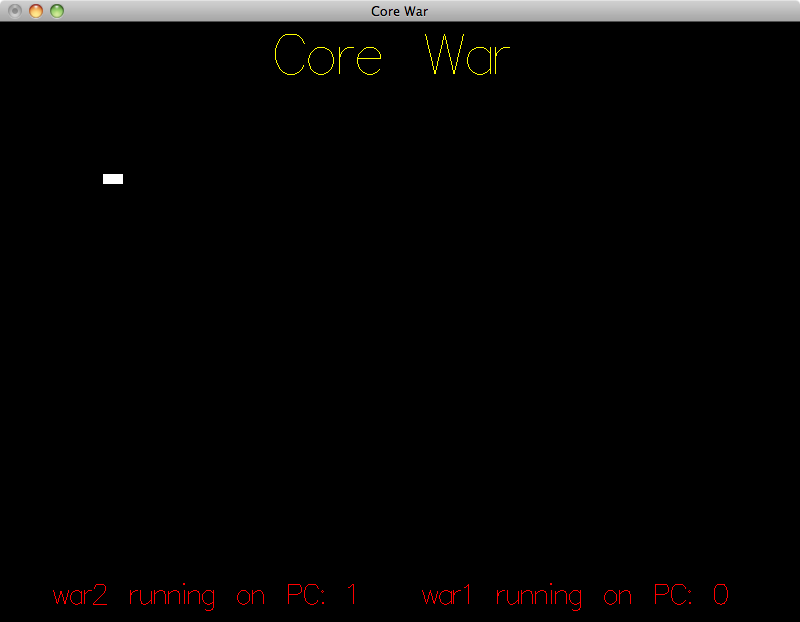
\includegraphics[height=90mm]{4}
			
\chapter{Problems encountered }
	\paragraph{}

\chapter{How we worked as a team}
	\paragraph{}...
	
\chapter{Conclusion}
	\paragraph{} We successfully implement the core war game, using haskell. And learning quite a lot for using gloss. We  worked as a team and met the basic requirements and as well as some additional ones.  

\chapter{References}
	\paragraph{}...			
			
\end{itemize}

\end{document}
